\chapter{World Objects Manipuleren}
\section{Object Classes en Code}
\subsection{Object Class}
Standaard is elk object in de game wereld een onderdeel van het terein. Dat betekent dat dit object op het scherm getoond zal worden, maar dat interactie met dat object niet mogelijk is. Wanneer je met een object meer wil doen dan het simpelweg tonen, dan is er een connectie nodig tussen het object en je code. Die connectie zag je eigenlijk al in het vorige hoofdstuk: daar maakten we een koppeling tussen een \texttt{OBJ\_PLAYER} en een de class \eeClass{player}.

Je gaat steeds op de volgende manier te werk:
\begin{enumerate}
	\item Maak een Object Class in de editor.
	\item Open je object en kies de tab Params. Daar kan je de Object Class instellen. (Zie afbeelding \ref{fig:objClass3})
	\item Schrijf de code voor je nieuwe class.
	\item Maak een \eeClass{Game.ObjMap} voor deze class.
	\item Link de Object Map aan de World.
\end{enumerate}
	
\begin{figure}[h]
\centering
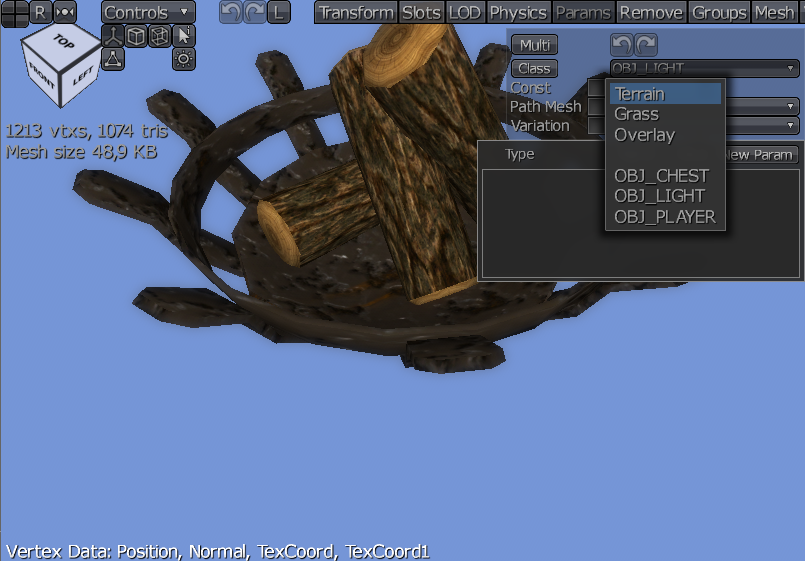
\includegraphics[width=0.8\linewidth]{../images/objClass3.png}
\caption[]{Een Object Class toewijzen.}
\label{fig:objClass3}
\end{figure}	

De eerste twee stappen spreken voor zich, dus we springen direct naar de derde stap.

\begin{note}
Start in dit hoofdstuk met de applicatie `3D World - stage 2'.
\end{note}

\subsection{Een custom object toevoegen}
\label{subsection:addObject}
Wanneer je de object class in de editor instelt, zal je zien dat het object niet meer in de wereld verschijnt als je je game start. Het object is immers geen onderdeel meer van het terrein, maar je hebt nog geen code geschreven om aan te geven wat er dan wel moet gebeuren. 

\begin{note}
Bij de game assets, in de map `other', vind je een object `magic lamp'. Er is ook al een object aanwezig in de game world. Dit object heeft de Object Class \texttt{OBJ\_MAGIC\_LAMP}. In deze oefening gaan we dat object rond zijn as laten draaien.
\end{note}

Wanneer je een class maakt voor een world object, dan moet je een speciale class als base class kiezen. Je hebt de keuze uit de volgende mogelijkheden:

\begin{itemize}
	\item \eeClass{Game.Animatable} gebruik je voor objecten met een animatie, zoals een kist die open en dicht kan.
	\item \eeClass{Game.Chr} gebruik je voor avatars, zoals de speler en mobs.
	\item \eeClass{Game.Destructible} gebruik je voor objecten die uiteen kunnen vallen in delen. (Op dit moment ontbreekt in de Editor een mogelijkheid om een dergelijk object te maken. Het kan wel via code, maar eenvoudig is dat niet.)
	\item \eeClass{Game.Door} gebruik je voor deuren.
	\item \eeClass{Game.Item} gebruik je voor voorwerpen waarmee interactie mogelijk is.
	\item \eeClass{Game.Static} gebruik je voor voorwerpen waarmee interactie mogelijk is, maar die op een vaste plaats blijven staan.
	\item \eeClass{Game.Kinematic} gebruik je voor voorwerpen waarmee interactie mogelijk is, maar die enkel via code verplaatst kunnen worden.
\end{itemize}

In deze oefening gebruiken we \eeClass{Game.Static}. Voorzie alvast de volgende class:

\begin{code}
class magicLamp : Game.Static {
	
}
Game.ObjMap<magicLamp> MagicLamp;
\end{code}

Pass in het bestand `main' de functie \eeFunc{Init()} aan:

\begin{code}
bool Init()
{
   Physics.create(EE_PHYSX_DLL_PATH);
   
   Game.World.activeRange(D.viewRange());
   Game.World.setObjType(Players, OBJ_PLAYER);
   Game.World.setObjType(MagicLamp, OBJ_MAGIC_LAMP); // <- New Code!
   Game.World.New(UID(2458107509, 1250513895, 1140948412, 2823156334));
   if(Game.World.settings().environment)Game.World.settings().environment->set();
   
   return true;
}
\end{code}

Wanneer je nu het programma uitvoert, dan zal je zien dat de lamp zichtbaar is. 

\subsection{Virtuele functies}
De reden waarom je een object class moet baseren op een van de beschikbare \eeClass{Game} classes, is dat deze classes virtuele functies bevatten (met het keyword \eeFunc{virtual}). Wanneer je de header file van \eeClass{Game.Static} bekijkt, dan zie je dat alle functies in de class virtueel zijn. Bovendien is \eeClass{Game.Static} gebaseerd op \eeClass{Game.Obj}, die ook nog eens heel wat virtuele functies bevat.

Deze functies zijn nodig omdat de engine je eigen class niet kent. Door je class te koppelen aan de game wereld in de Init functie hierboven, link je je class aan de World Manager. Maar die kan niet weten wat voor functies jij aan die class toevoegt. De World Manager zal daarom functies uitvoeren die w\'el bekend zijn, zoals \eeFunc{update()} en \eeFunc{drawPrepare()}.

Aangezien deze functies virtueel zijn, kan je ze overschrijven in een afgeleide class. Met andere woorden: de World Manager voert de \eeFunc{update()} functie van \eeClass{Game.Static} uit, tenzij je een functie met dezelfde naam voorziet in de afgeleide class. In dat geval wordt je eigen functie uitgevoerd.

\subsection{Rotatie}
We willen in deze oefening de lamp roteren rond zijn Y-as. Dat gebeurt door de rotatie aan te passen in de update functie. Je moet dus een eigen update functie toevoegen:

\begin{code}
class magicLamp : Game.Static
{
   virtual bool update()
   {
      return super.update();
   }
}
\end{code}

De functie verwacht een \eeClass{bool} als resultaat. We voeren in dit geval de \eeFunc{update()} functie van \eeClass{Game.Static} uit en geven dat resultaat als functieresultaat.

Om het object te roteren maken we gebruik van zijn \eeClass{Matrix}. Een \eeClass{Matrix} voor een object is een combinatie van drie vectoren: x, y en z om de rotatie van een object in 3D te bepalen. Daarnaast bevat de \eeClass{Matrix} ook nog een vector voor de positie. De schaal van het object kan afgeleid worden uit de grootte van de eerste drie vectoren.

Om een \eeClass{Matrix} te roteren, kan je gebruik maken van \eeFunc{rotatie} functies. In dit geval willen we een rotatie rond de Y-as, dus kan je de volgende code gebruiken:

\begin{code}
virtual bool update()
{
	Matrix m = matrix();
	m.rotateY(1 * Time.d());
	matrix(m);
	return super.update();
}
\end{code}

Deze code doet het volgende:
\begin{itemize}
	\item Maak een nieuw object van de class \eeClass{Matrix}, met de waarden van de huidige object matrix.
	\item roteer de matrix, rekening houdend met de tijdsdelta.
	\item Geef de object matrix de waarde van de geroteerde matrix.
\end{itemize}

Start je programma en controleer het resultaat. Je zal zien dat de lamp elke 5 seconden voorbijvliegt. Wat gaat er mis?

Als je een bewerking uitvoert op een matrix, dan is die van toepassing op alle onderdelen van die matrix, dus ook op zijn positie! We roteren dus ook de positie van het object in de 3D wereld. Ik heb je deze fout laten maken omdat je dit goed moet onthouden.

De oplossing bestaat er in de Matrix eerst te verplaatsen naar zijn nulpunt. Zowel schalen als roteren dient steeds op het nulpunt te gebeuren. Daarna verplaats je de matrix terug naar de oorspronkelijke positie:

\begin{code}
virtual bool update()
{
	Matrix m = matrix();
	m.move(-pos());
	m.rotateY(1 * Time.d());
	m.move(pos());
	matrix(m);
	return super.update();
}
\end{code}

De nodige stappen voor een rotatie zijn dus:
\begin{itemize}
	\item Maak een nieuw object van de class \eeClass{Matrix}, met de waarden van de huidige object matrix.
	\item Verplaats het object naar zijn negatieve positie.
	\item Roteer de matrix, rekening houdend met de tijdsdelta.
	\item Verplaats het object naar zijn oorspronkelijke positie.
	\item Geef de object matrix de waarde van de geroteerde matrix.
\end{itemize}

\begin{exercise}
\begin{enumerate}
	\item Zoek een functie om de matrix zowel op de X als de Y-as te roteren. Gebruik voor beide assen een andere rotatiesnelheid.
	\item Zoek een functie om de matrix te schalen. Laat het object langzaam groter en kleiner worden. Hint: je kan de functies \eeFunc{Sin()}, \eeFunc{Time.appTime()} en \eeFunc{Time.d()} gebruiken om de schaal te berekenen.
\end{enumerate}
\end{exercise}

\section{Draw Functies}
\subsection{De Renderer}

Om een 3D wereld te renderen, gebruiken we de volgende code:

\begin{code}
void Render() {
   Game.World.draw();
}

void Draw() {
   Renderer(Render);
}
\end{code}

De functie \eeFunc{Draw()} is je wel bekend. Maar waar we vroeger zelf objecten op het scherm tekenden, laten we nu de \eeFunc{Renderer()} zijn werk doen. (Je kan natuurlijk later nog steeds een Gui en 2D elementen over het resultaat van de Renderer tekenen.

Die renderer heeft een functie nodig om hem te vertellen wat hij moet doen. In dit geval is dat de functie \eeFunc{Render()}. Daarin geven we de renderer de opdracht om de game wereld te renderen. Ook hier kan je later extra code toevoegen als je game complexer wordt.

Een begrijpelijke misvatting is dat je er van uit gaat dat die wereld in \'e\'en keer wordt gerenderd. De \eeFunc{Draw()} functie roept de \eeFunc{Renderer()} aan, de \eeFunc{Renderer} voert de functie \eeFunc{Render()} uit, en die voert \eeFunc{Game.World.draw()} uit, niet? 	

Maar zo eenvoudig is het niet. Het renderen van een 3D beeld gebeurt in verschillende fasen, die allemaal hun eigen doel hebben. Zo zijn er fasen voor het renderen van alle objecten, het toevoegen van licht, het toevoegen van schaduw en nog veel meer. Een volledig overzicht vind je in de engine header Graphics\\Renderer:

\begin{code}
enum RENDER_MODE // Rendering Mode, rendering phase of the rendering process
{
   RM_SIMPLE        , // simple
   RM_EARLY_Z       , // early z
   RM_SOLID         , // solid
   RM_SOLID_M       , // solid in mirrors/water reflections
   RM_AMBIENT       , // ambient
   RM_OVERLAY       , // overlay mode for rendering semi transparent surfaces onto solid meshes (like bullet holes)
   RM_OUTLINE       , // here you can optionally draw outlines of meshes using 'Mesh::drawOutline'
   RM_BEHIND        , // here you can optionally draw meshes which are behind the visible meshes using 'Mesh::drawBehind'
   RM_FUR           , // fur
   RM_BLEND         , // alpha blending
   RM_SHADOW        , // shadow map    , render all shadow casting objects here using 'Mesh::drawShadow', if objects will not be rendered in this phase they will not cast shadows
   RM_STENCIL_SHADOW, // shadow stencil, render all shadow casting objects here using 'Mesh::drawStencilShadow', if objects will not be rendered in this phase they will not cast shadows
   RM_CLOUD         , // clouds
   RM_WATER         , // water surfaces
   RM_PALETTE       , // color palette #0 (rendering is performed using 'Renderer.color_palette'  texture)
   RM_PALETTE1      , // color palette #1 (rendering is performed using 'Renderer.color_palette1' texture)
   RM_PREPARE       , // render all objects here using 'Mesh::draw', and add all lights to the scene using 'Light*::add'

   RM_SHADER_NUM=RM_SHADOW+1, // all modes from RM_SIMPLE to RM_SHADOW are included in the 'MeshPart' shader technique lookup list
};
\end{code}

In elke fase zal de renderer alle objecten in de World Manager overlopen en kijken of er iets moet gebeuren voor dat object. Voor de objecten waar je zelf een class voor maakt, kan je de renderer vertellen wat er moet gebeuren.

Om dat te doen, moet je eerst de virtuele functie \eeFunc{drawPrepare} overschrijven. Deze functie bepaalt welke extra fases dat op dit object van toepassing zijn. Het resultaat van deze functie is een \eeClass{uint}, een unsigned integer. Omdat elke game class zelf al enkele fases voorziet, roep je eerst de \eeFunc{drawPrepare()} functie van de base class aan.

\subsection{Outline Rendering}
We zullen nu outline rendering toevoegen aan de lamp uit de vorige sectie. Voeg alvast deze functie toe aan de class \eeClass{magicLamp}:

\begin{code}
virtual uint drawPrepare()
{
	uint result = super.drawPrepare();
	\\ add your own rendering phases here
	return result;
}
\end{code}

\begin{exercise}
Voeg aan de class magicLamp ook een bool `selected' toe. In de update functie schrijf je code om te detecteren of de L-toets ingedrukt is. Als dat zo is, dan wordt selected true, in het andere geval is selected false.
\end{exercise}

Om outline rendering uit te voeren is het nodig om deze mode aan het resultaat toe te voegen. Dat kan door de volgende code aan drawprepare toe te voegen:

\begin{code}
if(selected) {
	 result |= IndexToFlag(RM_OUTLINE);
}
\end{code}

Maar dat is niet genoeg. We moeten nu ook de outline draw functie van \eeClass{Game.Static} overschrijven. Die functie bestaat, maar is leeg. Het is dus niet nodig om \eeFunc{super.drawOutline()} uit te voeren.

\begin{code}
virtual void drawOutline()
{
	mesh->drawOutline(BLUE, matrixScaled());
}
\end{code} 

\begin{exercise}
\begin{itemize}
\item Wat gebeurt er als je hierboven de functie \eeFunc{matrixScaled()} door \eeFunc{matrix()} vervangt? Waarom?
\item Maak gebruik van een \eeClass{Color} om de alpha waarde van de kleur te varie\"eren met de tijd. Hint: gebruik terug de functie \eeFunc{Sin()} in combinatie met \eeFunc{Time.appTime()}.
\end{itemize}
\end{exercise}

\subsection{Draw Behind}
Een andere render mode is \eeClass{RM\_BEHIND}. In deze sectie ga je zelf aan de slag om deze mode toe te passen op de Object Class \texttt{OBJ\_CHEST}. De stappenlijst vermeldt de hoofdzaken. De details kan je vinden in de secties hierboven.

\begin{enumerate}
	\item Controleer dat je assets de Object Class \texttt{OBJ\_CHEST} bevat.
	\item Open Assets $\Rightarrow$ other $\Rightarrow$ chest en kijk in de tab Params of de class correct ingesteld is.
	\item Open de World en zorg dat er ten minste \'e\'en chest in de wereld staat.
	\item Maak een class chest, gebaseerd op \eeClass{Game.Static}.
	\item Voorzie een \eeClass{Game.ObjMap} voor deze class.
	\item Link in de \eeFunc{Init()} functie deze object map aan \texttt{OBJ\_CHEST}.
	\item Voeg aan je class een bool selected toe.
	\item Voeg een update functie toe, waarin je selected true of false maakt naargelang de status van de C toets.
	\item Voeg een functie \eeFunc{drawPrepare()} toe, waarin je de render mode \texttt{RM\_BEHIND} toevoegt als selected true is.
	\item Voeg de functie \eeFunc{drawBehind()} toe. Daarin schrijf je de volgende code:
	
	\begin{code}
		mesh->drawBehind(Color(64, 128, 255, 255), Color(255, 255, 255, 0), matrixScaled()); 
	\end{code}
	
	\item Experimenteer met verschillende kleuren tot je een origineel resultaat krijgt.
\end{enumerate}

\section{Mousepointer to 3D}
\subsection{Voorbeeldcode}
hierboven `selecteerden' we een object door een toets in te drukken. Daarbij zag je dat alle objecten van een type geselecteerd werden. Wanneer je slechts \'e\'en object van een bepaalde class wil selecteren, dan zal je op een andere manier te werk moeten gaan. Je zou bijvoorbeeld de afstand tot de speler kunnen controleren, maar in dit deel bekijken we hoe je een object kan selecteren via de mouse pointer.

Om dat te doen moeten we als uitgangspunt de positie van de muis op het scherm nemen en een denkbeeldige lijn in de diepte van het scherm trekken. Wanneer een object deze lijn raakt, dan is er een selectie mogelijk. Deze methode is behoorlijk rekenintensief. Daarom is het geen goed idee om ze uit te voeren in de class van het object, want dan moet die lijn voor elk object van die class opnieuw gemaakt en gecontroleerd worden.

\begin{exercise}
\begin{enumerate}
	\item Open de applicatie `3D World - stage 3'. 
	\item Pas alvast de functie \eeFunc{update()} van de class \eeClass{magicLamp} aan. De bool `selected' dient tijdens elke update false te worden.
	\item Maak een class \eeClass{inputControl}, en daaronder een object van deze class.
	\item Voeg aan de class een functie \eeFunc{void update()} toe.
	\item Voer deze update functie uit in de main \eeFunc{Update()} functie. Het maakt niet zoveel uit waar je de functie plaatst, maar het moet in ieder geval na \eeFunc{Game.World.update()} gebeuren. (Die voert immers de update functie van elk object uit, en daar zet je selected steeds op false.)
\end{enumerate}
\end{exercise}

We beginnen met een `mouseover' effect. Dat wil zeggen dat we eenvoudigweg controleren of een muis over een lamp beweegt, zonder extra controles. Voeg in de update functie van inputControl de volgende code toe:

\begin{code}
   void update()
   {      
      // stop if a gui element is clicked
      if ((Gui.msLit() != null) && (Gui.msLit()->type() != GO_DESKTOP)) return;

      Vec pos, dir;      
      ScreenToPosDir(Ms.pos(), pos, dir);
			
      PhysHit selector;      
      if (Physics.ray(pos, dir * D.viewRange(), &selector))
      {
         if (magicLamp * lamp = CAST(magicLamp, selector.obj))
         {
            lamp.selected = true;
         }
      }
      
   }
\end{code}

Wat betekent dit allemaal? Eerst staat er deze regel:

\begin{code}
if ((Gui.msLit() != null) && (Gui.msLit()->type() != GO_DESKTOP)) return;
\end{code}

Op dit moment heeft je project nog geen Gui. Maar als dat wel zo zou zijn, dan wil je geen objecten selecteren als je bijvoorbeeld op een button klikt. Het probleem is dat onder die gui nog altijd je wereld zit, dus een mouseclick zou zonder deze regel zowel de gui als de selectie in de wereld be\"invloeden. Deze regel controleert eerst of er een Gui element actief is. Wanneer het type van dat element gelijk is aan \texttt{GO\_DESKTOP} dan klik je wat de gui betreft op een leeg element, met andere woorden de wereld. De regel hierboven zorgt ervoor dat de rest van de functie niet uitgevoerd wordt wanneer je niet op die desktop klikt.

\begin{code}
Vec pos, dir;      
ScreenToPosDir(Ms.pos(), pos, dir);
\end{code}

Hier maken we twee vectoren die nodig zijn om een denkbeeldige lijn door de wereld te trekken. We gebruiken de functie \eeFunc{ScreenToPosDir()} om de 2D positie van de muis om te zetten in een 3D startpositie en een richting waarin de lijn moet lopen.

\begin{code}
PhysHit selector;
\end{code}

De functie die de denkbeeldige lijn controleert, moet je laten weten wat er geraakt werd. Dat gebeurt via dit object.

\begin{code}
if (Physics.ray(pos, dir * D.viewRange(), &selector))
\end{code}

Hier vraag je aan de Physics engine om een lijn (ray) te trekken. Deze functie heeft 3 argumenten:

\begin{description}
	\item[pos] de startpositie.
	\item[dir] de richting waarin de lijn moet lopen. We willen geen oneindig lange lijn. Dat zou betekenen dat Physics oneindig ver moet blijven controleren op objecten wanneer er geen object op de lijn zit. Daarom vermenigvuldigen we de richting met de viewRange. De viewRange is de afstand tot waar objecten in je game zichtbaar zijn.
	\item[selector] dit is een referentie naar het \eeClass{PhysHit} object dat je hierboven maakte. Physics zal het eerste object dat op deze lijn staat doorgeven aan dit object.
\end{description}

\begin{code}
if (magicLamp * lamp = CAST(magicLamp, selector.obj))
\end{code}

Wanneer Physics iets gevonden heeft, dan zit er een object in de selector. Maar we weten nog niet welk object. Het zou kunnen dat het terrein werd gevonden, of eender welk object in je game. Daarom proberen we het object om te zetten (te `casten') naar een (pointer naar een) object van het de class \eeClass{magicLamp}. Als dat lukt, dan weet je zeker dat je met een object van het juiste type te maken hebt.

\begin{code}
lamp.selected = true;
\end{code}

Wanneer een lamp gevonden werd, dan wijzigen we de waarde van selected. Hierboven heb je tijdens elke update alle lampen de waarde \texttt{selected = false} gegeven. Door deze functie na de wereld update uit te voeren, wordt enkel de lamp waar nu de muis over zit, true.

\subsection{Het werkt niet!}
Wanneer je nu je app uitvoert, dan zal je merken dat de selectie niet werkt. Om te onderzoeken wat er fout gaat, kijk je in zo'n geval best de Physics na. Dat kan eenvoudig door een regel toe te voegen aan de \eeFunc{Draw()} functie:

\begin{code}
void Draw() {
   Renderer(Render);
	 if(Kb.b(KB_EQUAL)) Physics.draw();
}
\end{code}

Als je nu opnieuw je programma uitvoert en door de wereld loopt, dan zie je dat de contouren van alle Physics objecten zichtbaar zijn wanneer je op de = toets drukt. Deze code wil je niet in je uiteindelijke game, maar tijdens de ontwikkeling kan dit wel erg handig zijn. Loop nu opnieuw naar de lamp, en je zal zien dat de Physics ontbreken. 

Wanneer je een object importeert in Esenthel, dan wordt er niet vanzelf een Physics object gemaakt. Je kan dat wel eenvoudig zelf doen. Je opent het object in de editor en kiest de tab `Physics'. Rechts zie je de verschillende opties. Je kan zelf de meest geschikte vorm kiezen, maar denk er wel aan dat meer detail altijd meer rekenkracht vergt.

Eens je object van physics voorzien is, zal de bovenstaande code zonder problemen werken.

\begin{exercise}
	\begin{itemize}
		\item Voer de Physics ray enkel uit wanneer de L-toets ingedrukt werd.
		\item Pas de zoekafstand aan, zodat een lamp enkel gevonden wordt tot op 10 meter afstand.
	\end{itemize}
\end{exercise}






